\documentclass[11pt, oneside]{article}   	% use "amsart" instead of "article" for AMSLaTeX format
\usepackage{geometry}                		% See geometry.pdf to learn the layout options. There are lots.
\geometry{letterpaper}                   		% ... or a4paper or a5paper or ... 
%\geometry{landscape}                		% Activate for for rotated page geometry
%\usepackage[parfill]{parskip}    		% Activate to begin paragraphs with an empty line rather than an indent
\usepackage{graphicx}				% Use pdf, png, jpg, or eps� with pdflatex; use eps in DVI mode
								% TeX will automatically convert eps --> pdf in pdflatex		
\usepackage{amssymb}
\usepackage{amsmath}

\title{Flux in Space}
%\author{The Author}
%\section{}
% \subsection*{R code}
\date{}							% Activate to display a given date or no date

\graphicspath{{/Users/telliott_admin/Dropbox/Tex/png/}}

% \begin{center} 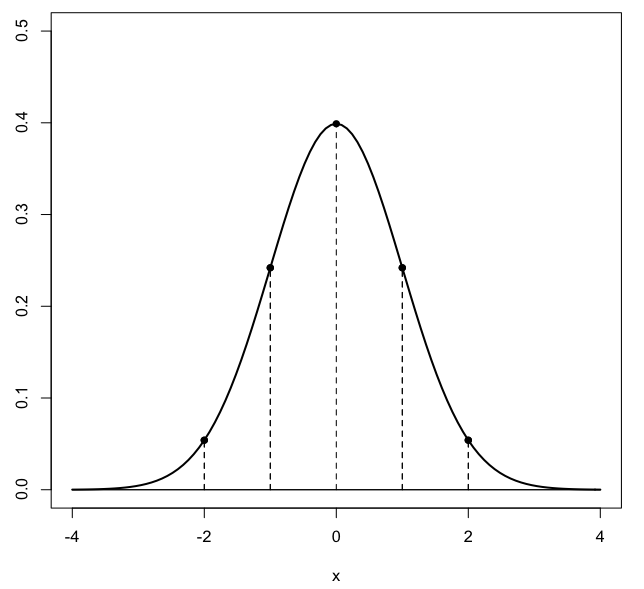
\includegraphics [scale=0.4] {gauss3.png} \end{center}
% \begin{bmatrix} a  &  b \\ c  &  d \end{bmatrix}
% \bigg |_

\begin{document}
\maketitle
\large
%\noindent

By now you should have seen Green's Theorem in the plane.
\[ \oint_C \mathbf{F} \cdot \mathbf{dr} = \oint_C \mathbf{F} \cdot \mathbf{\hat{t}} \ ds =  \iint\limits_{R}  curl(\mathbf{F}) \ dA \]
Often $curl(\mathbf{F}$ is written as $\nabla \times \mathbf{F}$.  If
\[  \mathbf{F} = \ <M,N> \ \]
then we have the equivalent expression
\[ \oint_C M \ dx + N \ dy  = \iint\limits_{R} (N_x - M_y) \ dA \]
remembering that the integral on the left is a single integral, so we must eventually get $x$ in terms of $y$ or both in terms of $t$ to use the formula.  There is a great trick where if $N_x = 1/2$ and $M_y = - 1/2$ then the right-hand side is
\[  \iint\limits_{R} (\frac{1}{2} - -\frac{1}{2}) \ dA = \iint\limits_{R} dA = A \]
and this leads to a simple calculation of the area of an ellipse.  More often, we can avoid a complicated line integral by converting it to the right-hand side.  And of course if $\nabla \times \mathbf{F} = N_x-M_y = 0$, we are dealing with a conservative vector field and we just evaluate the potential at the end-points of the curve, obtaining zero for the example with a closed curve.

An alternative version of Green's Theorem involves the divergence of $\mathbf{F}$
\[ Flux =  \oint_C \mathbf{F} \cdot \mathbf{n} \ ds = \iint\limits_{R} \nabla \cdot \mathbf{F} \ dx \ dy \]
where 
\[ div(\mathbf{F}) = \nabla \cdot \mathbf{F} = M_x + N_y \]
The term $\mathbf{F} \cdot \mathbf{n}\ ds$ is the orthogonal counterpart (flow across the curve) of $\mathbf{F} \cdot \mathbf{t} \ ds = \mathbf{F} \cdot \mathbf{dr}$, the work done along $C$.  $\mathbf{n}$ can be a little tricky to work with, but the point of this seems to be that we can convert the divergence (say, of a flow field) into a simpler calculation over the area of $R$.  For reference 
\[ \mathbf{n} = \frac{1}{| \mathbf{r}'(t) |} \ <\frac{dy}{dt},-\frac{dx}{dt} > \]
Velocity is in the direction we're headed $\mathbf{v} = \ <dx/dt,dy/dt>$.  This vector is orthogonal to it ($\mathbf{v} \cdot \mathbf{n} = 0)$, and it's a unit vector.
\subsection*{In space}
Moving on to the actual topic for this write-up, we start to think about space.  The flux of $\mathbf{F}$ across a surface $S$ is
\[ Flux =   \iint\limits_{S}  \mathbf{F} \cdot \mathbf{n} \ dS \]
where $\mathbf{n}$ is the unit normal to the surface.  Let's look more carefully at $ \mathbf{n} \ dS$.  Back when we looked at parametrization of surfaces, we said that
\[ dS = | \mathbf{r}_u \times \mathbf{r}_v | \ du \ dv \]
but the unit normal to the surface is just
\[ \mathbf{n} = \frac{\mathbf{r}_u \times \mathbf{r}_v}{|\mathbf{r}_u \times \mathbf{r}_v|} \]
so 
\[ \mathbf{n} \ dS = \mathbf{r}_u \times \mathbf{r}_v \ du \ dv \] 
and 
\[ Flux =   \iint\limits_{S}  \mathbf{F} \cdot \mathbf{n} \ dS =   \iint\limits_{S}  \mathbf{F} \cdot (\mathbf{r}_u \times \mathbf{r}_v) \ du \ dv \]
\subsection*{example}
Suppose we have a unit sphere 
\[ x^2 + y^2 + z^2 = 1 \]
and $\mathbf{F}= \ <x,y,z>$.
The standard parametrization of the (unit) sphere is
\[ \mathbf{r}(\phi, \theta) = \ <\sin \phi \cos \theta, \sin \phi \sin \theta, \cos \phi> \]
$\mathbf{F}$ is actually just the same.  The cross-product is
\[ \mathbf{r}_{\phi} \times \mathbf{r}_{\theta} =  \]
\[ \mathbf{r}_{\phi} = \ < \cos \phi \cos \theta, \cos \phi \sin \theta, -\sin \phi > \ \]
\[ \mathbf{r}_{\theta} = \ < \sin \phi \sin \theta, \sin \phi \cos \theta, 0 > \ \]
The cross-product is
\[ < -\sin^2 \phi \cos \theta, \sin^2 \phi \sin \theta, \sin \phi \cos \phi> \]
The dot product is
\[ \sin \phi \cos \theta \sin^2 \phi \cos \theta +  \sin \phi \sin \theta \sin^2 \phi \sin \theta + \cos \phi \sin \phi \cos \phi \]
\[ = \sin^3 phi + \sin \phi \cos^2 \phi = \sin \phi \]
So we have
\[ \int_0^{2\pi} \int_0^{\pi}  \sin \phi \  d \phi \ d \theta = \int_0^{2\pi} 2 \ d \theta = 4 \pi \]
\subsection*{divergence theorem}
There is an easier way to do this calculation!  It uses the divergence theorem in space, which states the following identity
\[ flux =  \iint\limits_{S}  \mathbf{F} \cdot \mathbf{n} \ dS = \iiint\limits_{V} div \mathbf{F} \ dV \]
Remember that
\[ \mathbf{F}= \ <x,y,z> \]
\[ div(\mathbf{F} ) = \nabla \cdot \mathbf{F} = P_x + Q_y + R_z = 1 + 1 + 1 = 3 \]
So we have
\[ = \iiint\limits_{V} 3 \ dV  = 3 V =  4 \pi \]


\end{document}  